\documentclass{standalone}
% main document, called main.tex

% \usepackage{newtxtext}       %
% \usepackage{newtxmath}      

\newcommand\szcirc{0.36cm}

\usepackage{tikz}

\begin{document}

\newcommand{\juv}{S}

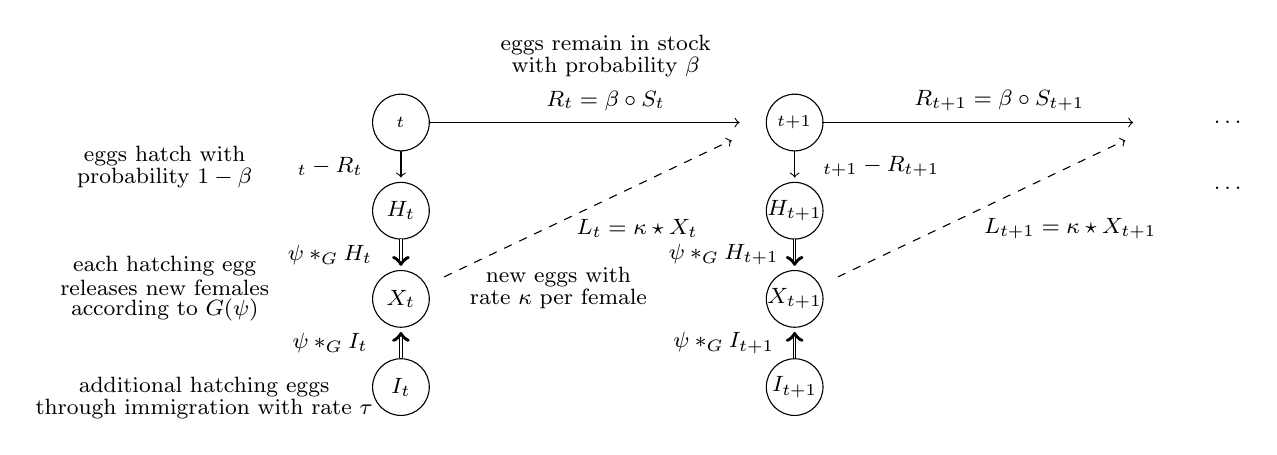
\begin{tikzpicture}[x=1cm,y=0.28cm]
\footnotesize
% two place holders to get some margins:
% \draw[white,fill=white](6,1) node {};
% \draw[white,fill=white](6,1) node {};

% circles:
\draw[black,fill=white](11,1) circle (\szcirc) node {$\juv_{t}$};
\draw[black,fill=white](11,-3) circle (\szcirc) node {$H_{t}$};

\draw[black,fill=white](11,-7) circle (\szcirc) node {$X_{t}$};
\draw[black,fill=white](11,-11) circle (\szcirc) node {$I_{t}$};

\draw[black,fill=white](16,1) circle (\szcirc) node {$\juv_{t + 1}$};
\draw[black,fill=white](16,-3) circle (\szcirc) node {$H_{t + 1}$};
\draw[black,fill=white](16,-7) circle (\szcirc) node {$X_{t + 1}$};
\draw[black,fill=white](16,-11) circle (\szcirc) node {$I_{t + 1}$};

% dots right
\draw[black,fill=white](21.5,1) node {$\dots$};
\draw[black,fill=white](21.5,-2) node {$\dots$};

% long horizontal arrows:
\foreach \x/\y in {11/15.3, 16/20.3}
{\draw[->] (\x.35,1) -- (\y,1);}


% vertical arrows:
\foreach \x in {11, 16}
{\draw[->] (\x, -0.3) -- (\x, -1.5);
\draw[->, double distance=0.5pt] (\x, -4.3) -- (\x, -5.5);
\draw[->, double distance=0.5pt] (\x, -9.7) -- (\x, -8.5);
}

% diagonal arrows:
\foreach \x in {11, 16}
{\draw[->, dashed] (\x + 0.55, -6) -- (\x + 4.2, 0.2);
}

% text
\draw[black,fill=white](8,-0.5) node {eggs hatch with};
\draw[black,fill=white](8,-1.5) node {probability $1 - \beta$};
\draw[black,fill=white](10.1,-1) node {$\juv_t - R_t$};
\draw[black,fill=white](17.1,-1) node {$\juv_{t + 1} - R_{t + 1}$};

\draw[black,fill=white](10.1,-5) node {$\psi *_G H_t$};
\draw[black,fill=white](15.1,-5) node {$\psi *_G H_{t + 1}$};

\draw[black,fill=white](8,-5.5) node {each hatching egg};
\draw[black,fill=white](8,-6.5) node {releases new females};
\draw[black,fill=white](8,-7.5) node {according to $G(\psi)$};

\draw[black,fill=white](10.1,-9) node {$\psi *_G I_t$};
\draw[black,fill=white](15.1,-9) node {$\psi *_G I_{t + 1}$};
\draw[black,fill=white](8.5,-11) node {additional hatching eggs};
\draw[black,fill=white](8.5,-12) node {through immigration with rate $\tau$};

\draw[black,fill=white](13.6,4.5) node {eggs remain in stock};
\draw[black,fill=white](13.6,3.5) node {with probability $\beta$};
\draw[black,fill=white](13.6,2) node {$R_t = \beta \circ S_t$};
\draw[black,fill=white](18.6,2) node {$R_{t + 1} = \beta \circ S_{t + 1}$};


\draw[black,fill=white](14,-3.8) node {$L_t = \kappa \star X_t$};
\draw[black,fill=white](13,-6) node {new eggs with};
\draw[black,fill=white](13,-7) node {rate $\kappa$ per female};
\draw[black,fill=white](19.5,-3.8) node {$L_{t + 1} = \kappa \star X_{t + 1}$};

\end{tikzpicture}

\end{document}